\documentclass[twocolumn]{article}
\usepackage[dvipdfmx]{graphicx}
\begin{document}

\title{Staged Training to ternarize neural network weight}
\author{Kenji Ogura}
\date{April 01 2020}
\maketitle

\section{Abstract}

For small device or Embedded systems without GPU, realtime object detection task via Neural Networks should be worked.
I was inspired below papers,
\begin{itemize}
\item
 Training a Binary Weight Object Detector byKnowledge Transfer for Autonomous Driving[1]
\item
 Ternary weight networks[2]
\item
 XNOR-Net: ImageNet Classification Using BinaryConvolutional Neural Networks[3]
\end{itemize}

Generally the inference task using full ternary weights -1,0,+1 is considered as low accuracy than full precision weights.
But for mobile device such as raspberryPI small weights will be efficiency choice.
Many quantization methods for model weights are proposed now such as FP16, bfloat, fixed point 16bits, 8bit, ternary 2bits and XNor 1bit too.
I consider that re-training after quatization of weights is needed.
How to train using some quantization methods? from ground, finetune?

\section{Staged training method}
In this paper I propose the staged training for yolov2-voc.cfg, yolov3-voc.cfg on Darknet website[4].
You can get full ternarized weights within 3 points accuracy drops for yolov2, within 4.5 points accuracy dorops for yolov3 using this method.
2bits ternary weights representaion is x8 smaller than 32bit floating point.

Staged training generates Ternarized weights for yolov2-voc, yolov3-voc.
This method sprits training step into 4 stages.

\begin{itemize}
\item Stage-0 : first few layers are ternarized.
\item Stage-1 : last few layers are ternarized.
\item Stage-2 : all layers without last layer are ternarized.
\item Stage-3 : full ternarized.
\end{itemize}

Weights used on each stages is imported from previous stage, such as stage-2 weights from stage-1.
o
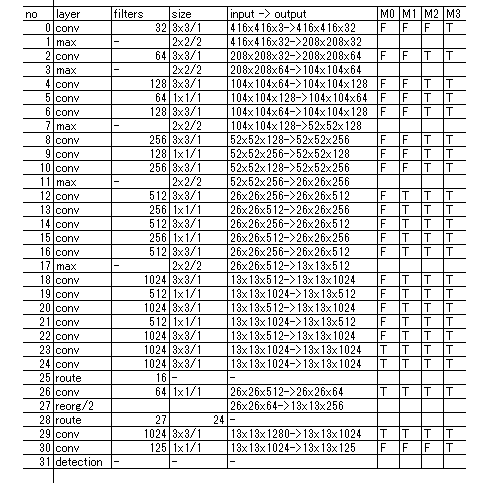
\includegraphics[width=10cm]{yolov2-voc_Stages.png}
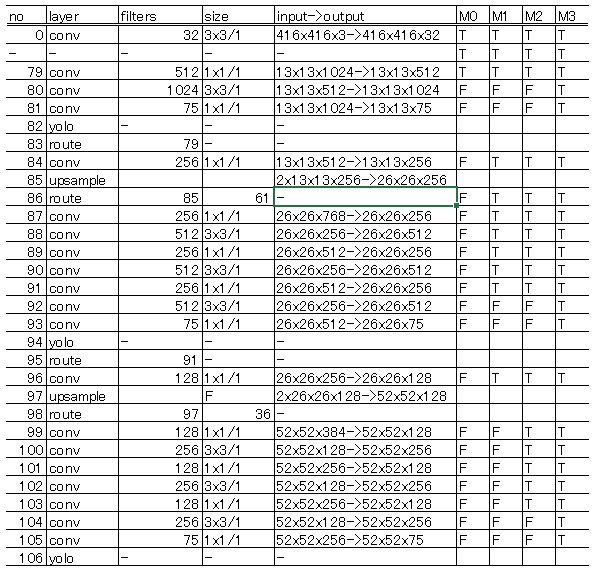
\includegraphics[width=8.5cm]{yolov3-voc_Stages.png}

We trained yolov2-voc.cfg on 4 jobs, and checked each loss curves.
And I use AlexeyAB[5] darknet to get mAP of experiments.
In fact, our experience denotes that accuracy via ternary weights drops about 3 points against full precision weights inferece.

\section{Result of Training}

Tables denote the result of staged training.
VOC 2012, 2007 Dataset is used with training and VOC 2007 for estimate of mAP.
Number of iteration is 40400, steps x0.1 at 80\%, 90\%, lr=0.001, burnin=1000 on Darknet framework.

\begin{table}[htbp]
 \centering
 \begin{tabular}{c|c|c|l}
  Stage & mAP & IOU & comments \\ \hline\hline
  -        & 76.85 & 54.67 & official Weights \\ \hline
  M0       & 77.09 & 57.04 & -                \\ \hline
  M1       & 76.44 & 56.18 & -                \\ \hline
  M2       & 75.06 & 57.71 & -                \\ \hline
  M3       & 73.82 & 54.90 & full ternary     \\ \hline\hline
 \end{tabular}
 \caption{result regard to yolov2}
 \label{tb:yolov2}
\end{table}

Iteration 41000(2000/class), steps x0.1 80\% 90\%, lr=0.001 at all stages

\begin{table}[htbp]
 \centering
 \begin{tabular}{c|c|c|l}
  Stage & mAP & IOU & comments \\ \hline\hline
  -        & 75.54 & 62.78 & FT from darknet53.conv.75 \\ \hline
  M0       & 75.02 & 63.04 & -                \\ \hline
  M1       & 73.69 & 63.75 & -                \\ \hline
  M2       & 73.76 & 63.54 & -                \\ \hline
  M3       & 71.26 & 61.61 & full ternary     \\ \hline\hline
 \end{tabular}
 \caption{result regard to yolov3}
 \label{tb:yolov3}
\end{table}

Iteration 100400(5000/class), steps x0.1 80\% 90\%, lr=0.001 at M0 and M1
Iteration 60400(3000/class), steps x0.1 80\% 90\%, lr=0.001 at M2 and M3

\begin{thebibliography}{99}
 \item Jiaolong Xu, Peng Wang, Heng Yang‡and Antonio et.al.
 "Training a Binary Weight Object Detector byKnowledge Transfer for Auonomous Driving" https://arxiv.org/pdf/1804.06332.pdf
 \item Fengfu Li and Bo Zhang, Bin Liu "Ternary weight networks" https://arxiv.org/pdf/1605.04711.pdf
 \item ohammad Rastegari, Vicente Ordonez, Joseph Redmon, Ali Farhadi Allen Institute for AI, University of Washington
 "XNOR-Net: ImageNet Classification Using BinaryConvolutional Neural Networks" https://arxiv.org/pdf/1603.05279.pdf
 \item https://github.com/pjreddie/darknet
 \item https://github.com/AlexeyAB/darknet

\end{thebibliography}

\end{document}
